% Options for packages loaded elsewhere
\PassOptionsToPackage{unicode}{hyperref}
\PassOptionsToPackage{hyphens}{url}
%
\documentclass[
  12pt,
]{article}
\usepackage{lmodern}
\usepackage{amsmath}
\usepackage{ifxetex,ifluatex}
\ifnum 0\ifxetex 1\fi\ifluatex 1\fi=0 % if pdftex
  \usepackage[T1]{fontenc}
  \usepackage[utf8]{inputenc}
  \usepackage{textcomp} % provide euro and other symbols
  \usepackage{amssymb}
\else % if luatex or xetex
  \usepackage{unicode-math}
  \defaultfontfeatures{Scale=MatchLowercase}
  \defaultfontfeatures[\rmfamily]{Ligatures=TeX,Scale=1}
\fi
% Use upquote if available, for straight quotes in verbatim environments
\IfFileExists{upquote.sty}{\usepackage{upquote}}{}
\IfFileExists{microtype.sty}{% use microtype if available
  \usepackage[]{microtype}
  \UseMicrotypeSet[protrusion]{basicmath} % disable protrusion for tt fonts
}{}
\makeatletter
\@ifundefined{KOMAClassName}{% if non-KOMA class
  \IfFileExists{parskip.sty}{%
    \usepackage{parskip}
  }{% else
    \setlength{\parindent}{0pt}
    \setlength{\parskip}{6pt plus 2pt minus 1pt}}
}{% if KOMA class
  \KOMAoptions{parskip=half}}
\makeatother
\usepackage{xcolor}
\IfFileExists{xurl.sty}{\usepackage{xurl}}{} % add URL line breaks if available
\IfFileExists{bookmark.sty}{\usepackage{bookmark}}{\usepackage{hyperref}}
\hypersetup{
  pdftitle={Tune Out or Turn Out? Covid-19 and the American Right},
  pdfauthor={Kevin Morris},
  hidelinks,
  pdfcreator={LaTeX via pandoc}}
\urlstyle{same} % disable monospaced font for URLs
\usepackage[margin=1in]{geometry}
\usepackage{longtable,booktabs}
\usepackage{calc} % for calculating minipage widths
% Correct order of tables after \paragraph or \subparagraph
\usepackage{etoolbox}
\makeatletter
\patchcmd\longtable{\par}{\if@noskipsec\mbox{}\fi\par}{}{}
\makeatother
% Allow footnotes in longtable head/foot
\IfFileExists{footnotehyper.sty}{\usepackage{footnotehyper}}{\usepackage{footnote}}
\makesavenoteenv{longtable}
\usepackage{graphicx}
\makeatletter
\def\maxwidth{\ifdim\Gin@nat@width>\linewidth\linewidth\else\Gin@nat@width\fi}
\def\maxheight{\ifdim\Gin@nat@height>\textheight\textheight\else\Gin@nat@height\fi}
\makeatother
% Scale images if necessary, so that they will not overflow the page
% margins by default, and it is still possible to overwrite the defaults
% using explicit options in \includegraphics[width, height, ...]{}
\setkeys{Gin}{width=\maxwidth,height=\maxheight,keepaspectratio}
% Set default figure placement to htbp
\makeatletter
\def\fps@figure{htbp}
\makeatother
\setlength{\emergencystretch}{3em} % prevent overfull lines
\providecommand{\tightlist}{%
  \setlength{\itemsep}{0pt}\setlength{\parskip}{0pt}}
\setcounter{secnumdepth}{5}
\usepackage{rotating}
\usepackage{setspace}
\usepackage{lineno}
\usepackage{booktabs}
\usepackage{longtable}
\usepackage{array}
\usepackage{multirow}
\usepackage{wrapfig}
\usepackage{float}
\usepackage{colortbl}
\usepackage{pdflscape}
\usepackage{tabu}
\usepackage{threeparttable}
\usepackage{threeparttablex}
\usepackage[normalem]{ulem}
\usepackage{makecell}
\usepackage{xcolor}
\ifluatex
  \usepackage{selnolig}  % disable illegal ligatures
\fi
\newlength{\cslhangindent}
\setlength{\cslhangindent}{1.5em}
\newlength{\csllabelwidth}
\setlength{\csllabelwidth}{3em}
\newenvironment{CSLReferences}[2] % #1 hanging-ident, #2 entry spacing
 {% don't indent paragraphs
  \setlength{\parindent}{0pt}
  % turn on hanging indent if param 1 is 1
  \ifodd #1 \everypar{\setlength{\hangindent}{\cslhangindent}}\ignorespaces\fi
  % set entry spacing
  \ifnum #2 > 0
  \setlength{\parskip}{#2\baselineskip}
  \fi
 }%
 {}
\usepackage{calc}
\newcommand{\CSLBlock}[1]{#1\hfill\break}
\newcommand{\CSLLeftMargin}[1]{\parbox[t]{\csllabelwidth}{#1}}
\newcommand{\CSLRightInline}[1]{\parbox[t]{\linewidth - \csllabelwidth}{#1}\break}
\newcommand{\CSLIndent}[1]{\hspace{\cslhangindent}#1}

\title{Tune Out or Turn Out? Covid-19 and the American Right}
\author{Kevin Morris\footnote{PhD Student, Department of Sociology, CUNY Graduate Center (\href{mailto:kmorris@gradcenter.cuny.edu}{\nolinkurl{kmorris@gradcenter.cuny.edu}})}}
\date{May 14, 2021}

\begin{document}
\maketitle
\begin{abstract}
The novel coronavirus SARS-CoV-2 (COVID-19) has upended normal routines across the United States. More than a half-million Americans have died of COVID-19, and more than 32 million have tested positive for the illness. In this short study, I argue that the failure of the Trump Administration can be understood through Max Weber's tripartite classification of legitimate domination. President Trump came to power by denigrating technical authority and celebrating charismatic leadership. The failure of this leadership may have led to a crisis among Trump supporters with closest contact with the virus---the sort of crisis Émile Durkheim indicates can result in either integrative of disintegrative impulses. Using national survey data, I show that COVID-19 contact among middle-of-the-road conservatives was associated with lower abstention and higher support for Biden, while such contact among very conservative Americans was associated with higher abstention but unrelated with presidential vote choice.
\end{abstract}

\pagenumbering{gobble}
\pagebreak

\pagenumbering{arabic}
\doublespacing

On January 21, 2020, the first case of SARS-CoV-2 (or ``COVID-19'') was confirmed in the state of Washington (\protect\hyperlink{ref-McNerthney2020}{McNerthney 2020}). President Donald Trump made his first public comments on the new virus the next day from Davos, telling CNBC ``we have it totally under control. It's one person coming in from China, and we have it under control'' (\protect\hyperlink{ref-Calia2020}{Calia 2020}). A few days later, on January 30, he said at a manufacturing plant in Michigan that ``we think we have it very well under control,'' assuring listeners that ``it's going to have a very good ending for it'' (\protect\hyperlink{ref-whitehouse2020}{{``Remarks by {President Trump} at a {USMCA Celebration} with {American Workers} \textbar{} {Warren}, {MI}''} 2020}). Meanwhile, cases were identified in states across the country. The first confirmed death attributed to COVID-19 occurred in Northern California on February 4th (\protect\hyperlink{ref-Moon2020}{Moon 2020}). By early March, Washington State was being called the center of the outbreak in the United States (\protect\hyperlink{ref-Golden2020}{Golden 2020}), although New York City would soon claim that dubious honor. By the time of the 2020 presidential election, more than 8.3 million Americans had tested positive for the novel coronavirus, with more than 220 thousand dead (\protect\hyperlink{ref-nyt2020}{\emph{New York Times: U.S.} 2020}). Reporting from a few months earlier, however, indicates that the official reports may be undercounts (\protect\hyperlink{ref-Lu2020}{Lu 2020}).

Although the World Health Organization declared COVID-19 a pandemic on March 11 (\protect\hyperlink{ref-Wan2020}{Wan 2020}), the response from the United State's federal government was slow. In the months to come, the Trump Administration would push responsibility to states and local governments, downplay the severity of the pandemic, and argue against the widespread stay-at-home orders promoted by public health experts (\protect\hyperlink{ref-Shear2020}{Shear et al. 2020}). Much of the United States remained at home throughout the summer even as peer nations were able to return to more normal daily life (\protect\hyperlink{ref-Douglas2020}{Douglas 2020}). The Trump Administration's response to the pandemic has consistently been criticized in the press, with Time Magazine reporting that a ``complete catalog of Trump's failures to adequately address the pandemic is the stuff of books, not single articles'' (\protect\hyperlink{ref-Fitzpatrick2020}{Fitzpatrick 2020}).

This project is interested in how voters react when their leader has failed them. I focus in particular on the behavior in the 2020 election of Republicans (and, more generally, conservatives) who were diagnosed with COVID-19, or knew someone who was diagnosed with or died from COVID-19. Given the popular reporting that ascribed much of the pandemic's severity to the Trump Administration, did these would-be voters opt out of participating at all, or did they support the opposing candidate? Put differently: did the tension between a party leader downplaying a pandemic with which they had deep personal experience lead to \emph{antisocial withdrawal}, or to \emph{prosocial engagement} with a different party?

I approach this question by reading classical sociological theorists alongside contemporary political science research. I begin by considering President Trump in the context of Max Weber's writings on charismatic leaders, and consider how the charismatic leader's failure---coupled with the systematic undermining of other bases of legitimacy---might leave those with the closest COVID contact adrift. Durkheim acknowledges that this might lead to anomie, and recent work in political science informs expectations about the particular groups for which COVID likely suppressed turnout.

Ultimately, I find that conservatives taken as a whole are both more likely to abstain \emph{and} more likely to support Biden when they have exposure to COVID-19. This rough cut, however, disguises variation within the Republican party's ideological camps. While moderate conservatives are \emph{motivated} to vote for Biden when exposed to COVID-19, far-right Americans withdrew from political participation at high rates in the face of this contradiction.

\hypertarget{trumpian-charisma}{%
\section*{Trumpian Charisma}\label{trumpian-charisma}}
\addcontentsline{toc}{section}{Trumpian Charisma}

Donald Trump's rise to the political power charted a path unique in American history. As Max Weber described more than a century ago, legitimate power is based on one of three characteristics: the leader must claim legitimacy on legal / rational, traditional, or charismatic grounds. Trump had neither the technical expertise in governance that might allow him to claim legal authority, nor was he part of the traditional coterie of the Republican Party like his competitors such as Jeb Bush or Newt Gingrich. With the two former avenues thus closed, Trump was left with only charisma --- a path for which he was uniquely situated. In \emph{The Sociology of Charismatic Authority} (2013), Weber explains: ``The charismatic leader gains and maintains authority solely by proving his strength in life'' (page 249). Charismatic leaders, he writes, are ``neither officeholders nor incumbents of an `occupation' in the present sense of the word, that is, men who have acquired expert knowledge and who serve for remuneration'' (245). Rather than appeal to those they lead on rational or technical grounds, the charismatic leader appeals to their ideals, base or otherwise.

Authority does not, of course, operate in a vacuum. To consolidate his own, charismatic authority, Trump immediately set out to undermine other forms of legitimate claims to power. This was first seen in his denigration of long-time public servants and his campaign promises to ``drain the swamp'' (\protect\hyperlink{ref-Shear2016}{Shear and Harris 2016}). In fact, much of Trump's campaign strategy was centered on casting himself as an outsider---in other words, he explicitly disavowed any claim to legitimacy based on tradition. His administration was largely staffed by individuals with little experience, thus removing individuals with competing claims to authority from high-level positions in the federal government.

While much has been made of President Trump's sidelining of individuals with potential claims to traditional authority, his undermining of legal or technical authority was no less important. Nowhere was this undermining more apparent prior to the advent of COVID-19 than in what became known as ``SharpieGate.'' On September 1, 2019, Hurricane Dorian was threatening the Southeastern United States. In advance of U.S. bound hurricanes, professional meteorologists at the National Oceanic and Atmospheric Administration (NOAA) make scientific predictions about what populations will likely be impacted by a coming storm. At a press conference, however, President Trump publicly contradicted experts at NOAA about the path of Hurricane Dorian, arguing that more people were in danger than the agency forecast (\protect\hyperlink{ref-Gonzales2019}{Gonzales 2019}). While telling people who were in no real danger to prepare for a hurricane might be bad politics in an immediate sense, actions such as these belie the project underlying all of President Trump's politics: by forcing voters to either listen to him or professional experts---whose legitimacy is based on technical / legal grounds---he consolidates his own claims to charismatic authority. Trump's authority is challenged by belief in any bases of legitimacy other than his own; he must therefore undermine the validity of any other claims to authority.

Trump's resistance to professionals' appeals to authority on legal, rational grounds takes on a new dimension in the context of COVID-19. Virology and disease, while socially mediated, are not responsive to charismatic leadership. The scientific community---and, more specifically, public health officials---were those with the skills needed to keep the American populace safe. These experts, however, could claim a legitimacy in direct opposition to Trump's. Moreover, it was a presidential election year. President Trump was faced with a choice: he could either acknowledge the legitimacy of legal, technical authority, or he could continue to undermine this authority as a legitimate basis for leadership. He chose to undermine these experts. By consistently downplaying the severity of the pandemic and casting doubt on technical experts' communications about the risk of the virus, he consolidated his claims to legitimacy. This contradiction was highly publicized: ``\,`Don't Be Afraid of Covid,' Trump Says, Undermining Public Health Messages'' read a typical headline from the \emph{New York Times} (\protect\hyperlink{ref-Kolata2020}{Kolata and Rabin 2020}).

But what happens when the emperor has no clothes? How do supporters of the charismatic leader respond when the sidelining of technical authority leads their acquaintances to get sick---and even to die? Do they turn to his competitor, or do they withdraw from political life?

\hypertarget{durkheim-and-social-solidarity}{%
\section*{Durkheim and Social Solidarity}\label{durkheim-and-social-solidarity}}
\addcontentsline{toc}{section}{Durkheim and Social Solidarity}

Predicting the likely behavior of Republican and conservative Americans who had personal contact with COVID-19 requires understanding when individuals withdraw from civil society and when they change their allegiance to a competing potential leader. Throughout his work, Émile Durkheim takes up the challenge of empirically measuring social cohesion, often using suicide rates as a proxy for overall solidarity. In \emph{The Division of Labor in Society} and \emph{Suicide}, Durkheim develops his theory of social solidarity. Social solidarity, he maintains, can be measured inversely by suicide. Although Durkheim ultimately identifies four types of suicide, we are here interested in just two: \emph{egoistic} and \emph{anomic} suicide.

Durkheim argues that suicide increases when the collective control over individuals' lives decreases. He traces the gradual lessening of mechanical solidarity over the centuries preceding his scholarship, theorizing that as the power of dominant structures such as the institutional Church waned, suicide would increase. When individuals are no longer constrained as part of a collective, \emph{egoistic} suicide increases. Communal care breaks down, and loneliness abounds. Egoistic suicide \emph{declines}, however, in times of political crisis. In these moments, the strength of the state is revealed, and social disintegration is at least temporarily reversed. These moments can ``rouse collective sentiments, stimulate partisan spirit and patriotism, political and national faith alike, and concentrating activity toward a single end, at least temporarily cause a stronger integration of society'' (page 208). In some key ways, the coronavirus pandemic can easily be understood from this perspective. Strong legal and normative rules were quickly established; behavior and movement was strictly monitored in many places; and public health messages broadly communicated that Americans were responsible for one another's health. Of course, not all Americans took the virus so seriously; in fact, it was highly politicized. Conservatives, who were generally more skeptical of the virus and organized political actions against government restrictions (e.g. \protect\hyperlink{ref-Bogel-Burroughs2020}{Bogel-Burroughs and Peters 2020}), may not have been roused in the same way. Nevertheless---as these anti-lockdown protests themselves demonstrate---aspects of the pandemic led to collective, integrative political action. Given these conditions, it seems possible that the pandemic could have resulted in stronger integration, and lower social withdrawal.

Although Durkheim argues that political crises can spur integration, he goes on to argue that other types of crisis---namely, economic ones---\emph{speed} social disintegration and increase suicide. Importantly, these economic disturbances need not be primarily negative to encourage the suicidal tendency. ``Every disturbance of equilibrium,'' Durkheim writes, ``even though it achieved greater comfort and a heightening of general vitality, is an impulse to voluntary death'' (page 246). When individuals' expectations for the future fall out of balance, when they feel as though they cannot understand the rules of the game they are playing, anomie increases. This may have been the case for many Americans in the face of the coronavirus---particularly for conservatives with direct contact with the virus. They supported a charismatic leader who vehemently undermined technical experts, but that leader was incapable of keeping them safe. The tools they used to understand the world were failing; they could either continue to support an administration that had caused the illness or death of someone they knew, or they could withdraw even more from the body politic.

Of course, economic and political crises are hardly mutually exclusive. Durkheim's theory of the relationship between crisis and social solidarity is therefore at least partially contradictory. The COVID-19 pandemic, then, points us to a tension at the heart of Durkheim's writing about social solidarity: the same event can contain pushes to both anti- and prosocial behavior. This tension between Durkheim's assertion that \emph{political} crises lead to lower suicide while \emph{economic} one lead to higher suicide has been noted by \protect\hyperlink{ref-Pope1975}{Pope} (\protect\hyperlink{ref-Pope1975}{1975}) and others. The politics around COVID-19 make the pandemic an ideal forum in which to test what psychological mechanisms lead to integration---and, more generally, when crisis leads to cohesion. Throughout the remainder of this piece, voting will be considered a proxy for pro-social behavior; abstention, on the other hand, will play for us the same theoretical role that suicide played for Durkheim. As noted above, I focus in particular on conservatives who report contact with COVID-19; these are the individuals for whom this tension in Durkheim's theory is most urgent.

The responses we expect to see are not altogether predictable. There is a remarkable lack of literature in political science on what leads registrants of one party to support the candidate of another, especially in a specifically American context \protect\hyperlink{ref-Bakker2016}{Bakker et al.} (\protect\hyperlink{ref-Bakker2016}{2016}). Where the question has been considered, the distinction between abstention and supporting another party's candidate has been largely collapsed: a loyalist ``leaves no stone unturned before he resigns himself to the painful decision to \emph{withdraw or switch}'' reads a typical description (\protect\hyperlink{ref-Hirschman1970a}{Hirschman 1970, 83}, emphasis added). Are strong party loyalists most exposed to the failures of their party's standard bearer---as very conservative Americans with a front-row seat to COVID-19 could be considered---\emph{more} likely to see collective sentiments roused than others with weaker partisan identities? Or will the enormous disruption of the virus, coupled with perceived abandonment from the top, lead them to withdraw?

While little work has directly explored when voters abstain or defect to the opposite party's candidate, a large body of literature exploring the role of partisanship in social life can help shed some light on the question. Recent work from political scientists has detailed just how deeply American's partisan commitments run (\protect\hyperlink{ref-Iyengar2019}{Iyengar et al. 2019}; \protect\hyperlink{ref-Mason2018}{Mason 2018}). A growing body of literature indicates that voting is more often an \emph{expressive} act than it is a purely rational act driven by expected policy outcomes (\protect\hyperlink{ref-Green2002}{Green, Palmquist, and Schickler 2002}). The expressive model of voting, built on social identity theory, holds that partisanship is a central aspect of Americans' social identities, much like religion or race. Under this model, an individual supports a given politician less because of their stance on given issues than because they feel they represent their ``team.'' \protect\hyperlink{ref-Huddy2015}{Huddy, Mason, and Aarøe} (\protect\hyperlink{ref-Huddy2015}{2015}), for instance, demonstrates that individuals who strongly identify as partisans are angier when faced with electoral loss, and happier after an electoral win, than voters with consistent ideological stances across a range of issues---voters whose policy preferences ``should'' mean they care more about who is elected. As Mason (\protect\hyperlink{ref-Mason2015}{2015, 128}) puts it, the United States is ``a nation that agrees on many things but is bitterly divided nonetheless.'' These deep divisions, even among Americans who support similar policies, provides strong evidence that partisan identity is a different beast than policy preferences. In short, partisan identity ``is a deep-seated psychological predisposition, which is both stable and drives most of the core political decisions we make'' (\protect\hyperlink{ref-Abrajano2017}{Abrajano and Hajnal 2017, 15}).

Given this context, it seems highly likely that strong conservatives could not easily switch parties in response to COVID-19. Put differently, they probably saw no avenue through which their sentiments could productively be channeled. This becomes clearer when we turn once again to Weber. The Trump presidency was not just a contest over policy ideas and goals, but rather the bases of legitimacy. Ardent Trump supporters could not, therefore, support Biden without effectively renouncing their understanding of the ordering of political power. Less-strongly committed conservatives, on the other hand, might have supported Trump because of his policy objectives but \emph{in spite of} the basis of his claims to authority. The threat posed by contact with COVID-19 may have spurred these individuals to action---and even to support a liberal presidential candidate. In short, the 2020 election allows me to test how group affiliation and exposure to threat structures anomie and the attendant social withdrawal.

\hypertarget{data-and-hypotheses}{%
\section*{Data and Hypotheses}\label{data-and-hypotheses}}
\addcontentsline{toc}{section}{Data and Hypotheses}

To test the effect of partisan identity and exposure to COVID-19, I leverage data from the 2020 Cooperative Election Study (CES, formerly known as the Cooperative Congressional Election Study). The CES is fielded each year, with a pre- and post-wave in even-numbered years. In 2020, the CES surveyed 61,000 individuals, asking a host of questions about voters sociodemographic characteristics, partisan affiliations, and voting behavior. The sample is weighted to be representative of all American adults, not just voters or registered voters. In 2020, the CES also asked questions specifically about respondents' exposure to COVID-19. They ask about whether respondent or anyone they knew had been \emph{diagnosed} with COVID-19, as well as whether anyone they knew died from the illness.

To test whether voters were more likely to opt-out or to support a candidate of a different party, I run a multinomial logistic model, where the dependent variable takes one of three values: ``Did not vote''; ``Voted for Party's Candidate''; and ``Voted for Another Candidate.'' The primary independent variables are exposure to COVID-19, and I include a number of standard covariates which include party identification; race; age; gender; education level; household income; presidential vote choice in 2016; and a 7-point scale of ideology. Finally, to test the different effects of COVID-19 exposure for different parties, exposure is interacted with party identification.

These models allow me to test the following hypotheses:

\textbf{H1:} Registered Democrats who knew someone diagnosed with or who died from COVID-19 were more likely to vote, other things equal. Republicans with exposure to COVID-19, on the other hand, were less likely to vote.

\textbf{H2:} Exposure to COVID-19 decreased Republicans' likelihood of voting for Trump, while it increased the probability that Democrats voted for Biden. However, because partisan identity is so sticky, I expect that COVID-19 exposure had less of an effect on vote-choice than whether an individual participated. Put differently, I expect that Republicans were more likely to abstain from voting than to switch parties in the face of COVID-19.

The CES also includes self-reported measures of ideology, ranging on a 7-point scale from ``very liberal'' to ``very conservative.'' To better understand the relationship between party loyalty, withdrawal, and COVID-19 I estimate the same model as that described above, but here investigate whether contact with COVID-19 differently structured turnout and vote choice \emph{within} the conservative population. I expect that ``somewhat conservative'' voters will be more likely to switch to support Biden, while ``very conservative'' voters will abstain at higher rates. Put formally, I test the following hypothesis:

\textbf{H3:} Other things being equal, contact with COVID-19 will result in substantially higher abstention rates for ``very conservative'' voters than for other conservatives.

\hypertarget{results}{%
\section*{Results}\label{results}}
\addcontentsline{toc}{section}{Results}

Before proceeding to the econometric modeling, I present the results of the characteristics of survey respondents with contact with COVID-19.\footnote{Respondents report their incomes in bucketed groups (e.g.~``Between \$40,000 and \$50,000''). These incomes are re-coded as the midpoint of each range.} These characteristics are presented in Table \ref{tab:demos}.

\begin{singlespace}
\begin{table}[!h]

\caption{\label{tab:balance-tab-full}\label{tab:demos} Group Contact with COVID-19}
\centering
\begin{tabular}[t]{lcc}
\toprule
\multicolumn{1}{c}{ } & \multicolumn{2}{c}{Knew Someone Who...} \\
\cmidrule(l{3pt}r{3pt}){2-3}
Group & Died & Was Diagnosed\\
\midrule
\addlinespace[0.3em]
\multicolumn{3}{l}{\textbf{Race}}\\
\hspace{1em}Asian & 11.7\% & 42.0\%\\
\hspace{1em}Black & 20.8\% & 48.7\%\\
\hspace{1em}Latinx & 20.5\% & 53.5\%\\
\hspace{1em}Other Race & 16.6\% & 51.4\%\\
\hspace{1em}White & 12.5\% & 50.2\%\\
\addlinespace[0.3em]
\multicolumn{3}{l}{\textbf{Party}}\\
\hspace{1em}Democrat & 18.6\% & 55.4\%\\
\hspace{1em}Republican & 10.9\% & 45.5\%\\
\hspace{1em}Other Party & 13.3\% & 48.5\%\\
\addlinespace[0.3em]
\multicolumn{3}{l}{\textbf{Income}}\\
\hspace{1em}Less than \$50k & 12.6\% & 43.2\%\\
\hspace{1em}\$50k - \$100k & 15.8\% & 54.6\%\\
\hspace{1em}More than \$100k & 18.5\% & 61.5\%\\
\addlinespace[0.3em]
\multicolumn{3}{l}{\textbf{Age}}\\
\hspace{1em}Less than 45 & 13.3\% & 51.6\%\\
\hspace{1em}45 - 64 & 16.5\% & 51.7\%\\
\hspace{1em}65 or Older & 13.8\% & 44.6\%\\
\bottomrule
\end{tabular}
\end{table}
\end{singlespace}

Table \ref{tab:demos} shows that there were meaningful group-level differences in COVID-19 contact. Surprisingly, these vary based on whether we look at COVID-19 diagnoses or deaths. White respondents, for instance, were slightly more likely to know someone who was \emph{diagnosed} with COVID-19 than Black respondents, but were substantially less likely to know someone who \emph{died} from the disease. Higher-income respondents were also much more likely to report knowing someone who was diagnosed with or died from COVID-19 than middle- and low-income respondents. Public reporting indicates that the disease was actually more common among lower-income and non-white populations, so these patterns are somewhat surprising. The same is true of the age patterns, in which older individuals were not more likely to know people who had contracted or died of COVID-19. Nevertheless, as we are interested in how individuals' \emph{own experience} of the disease influenced their behavior, we use these self-reported contact measures.

I begin by running two mulitnomial logistic regressions. The dependent variable takes 1 of 3 values: voted for in-party candidate; voted for out-party candidate; and abstained (for non-partisan respondents, any vote is considered out-party). The primary independent variables are dummies indicating whether the respondent knew anyone diagnosed with COVID (in model 1) or who died from COVID (in model 2). These dummies are interacted with partisan identification dummies to measure whether the effect of contact was different for members of different political parties.

Because the results of the mulinomial logistic regressions are difficult to interpret directly, I here present the marginal effects plots for these models (the full tables can be found in the Supplemental Information). All other covariates are held at their means. The top panels present the results from model 1 (where I measure the effect of knowing someone diagnosed with COVID) while the bottom panels show the results of model 2 (that is, the effect of knowing someone who died from COVID). The left-hand panels measure show whether contact was associated with abstention (that is, not voting), and the right-hand panels show the effect of contact on voting for the other party's presidential candidate. Because the options are binary for unaffiliated voters (vote or abstain) I do not plot their behavior in the right-hand panels; their vote behavior is the inverse of their behavior in the left-hand panels.

\begin{figure}[!htbp]

{\centering 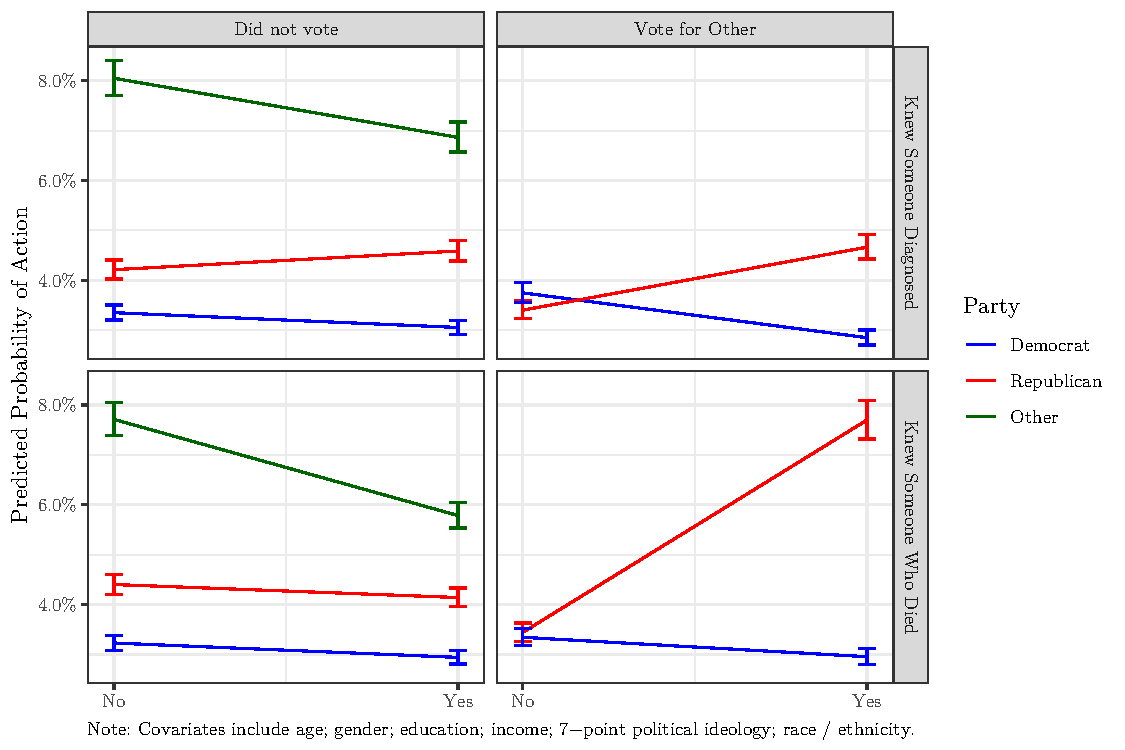
\includegraphics{theory_paper_files/figure-latex/mef1-c-1} 

}

\caption{\label{fig:mef1}Predicted Behavior, 2020 Election}\label{fig:mef1-c}
\end{figure}

Figure \ref{fig:mef1} makes clear that contact with individuals who were diagnosed with or died from COVID-19 did structure political behavior, and that the effect differed by party affiliation. While contact with someone diagnosed with COVID-19 \emph{decreased} the abstention rate for Democrats and unaffiliated voters, it \emph{increased} the abstention rate of Republicans by about 11 percent, relative to voting for Trump. Contact with someone diagnosed also increased the probability that both Democrats and Republicans voted for Biden by a considerable amount.

Knowing someone who died from COVID-19 had similar effects to those of knowing someone diagnosed for Democrats and unaffiliated voters. They were less likely to abstain and more likely to support Biden. The relative effect sizes, however, shift dramatically for Republicans. The ``strong'' treatment of knowing someone who died from COVID-19 slightly decreased Republicans' abstention rate, and was associated with a \emph{far} higher probability of voting for Biden. In fact, Republicans who knew someone who died of COVID-19 were more than twice as likely to vote for candidate other than Trump, all else equal and relative to supporting Trump. It seems, then, that the ``weaker'' treatment of knowing someone diagnosed with COVID-19 led Republicans to withdraw; the ``stronger'' treatment, however, led them to support an opposing candidate.

Of course, party identification is a very rough grouping: with just two major parties in the United States, each party includes a broad swath of voters. However, because the CES includes self-reported measures of partisanship, I can test whether an individual's position \emph{within} the conservative landscape is associated with their reaction to COVID-19 in 2020. I re-run similar models to those discussed above. Here, however, I regress vote choice / abstention not on a voter's party affiliation, but on their self-reported ideology. Once again, model 1 tests the effect of knowing someone diagnosed, while model 2 tests the effect of knowing someone who died from COVID-19. As before, I include in the body of this paper only the marginal effects plot; the full table can be found in the Supplementary Information.

Although these models include all voters, I am primarily interested in the behavior of conservatives. As such, Figure \ref{fig:mef2} plots only the effect of contact with COVID-19 on the behavior of self-identified conservatives. Once again, all covariates are held at their means.

\begin{figure}[H]

{\centering 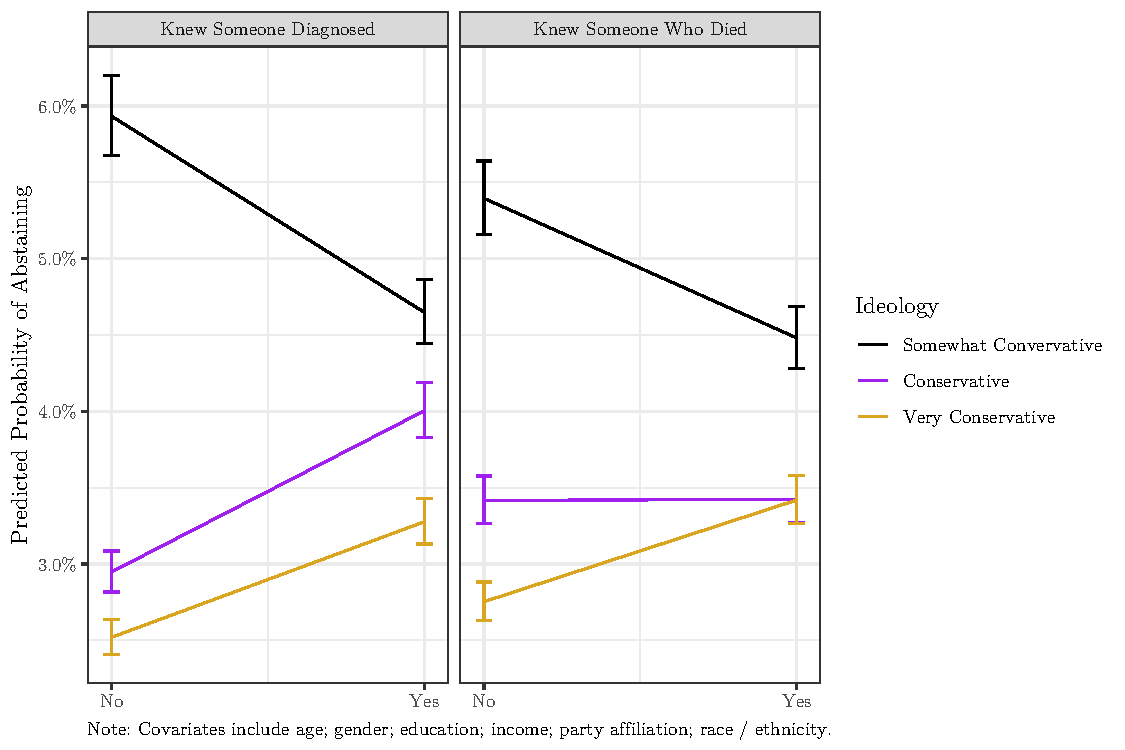
\includegraphics{theory_paper_files/figure-latex/mef2-c-1} 

}

\caption{\label{fig:mef2}Predicted Behavior of Conservatives, 2020 Election}\label{fig:mef2-c}
\end{figure}

Figure \ref{fig:mef2} shows similar trends to those in Figure \ref{fig:mef1}. While ``somewhat conservative'' voters were motivated to vote by having contact with someone with COVID-19, the opposite was true for ``very conservative'' individuals. These respondents were far more likely to withdraw from the political process altogether. The behavior of the middle-of-the-road conservatives is perhaps the most interesting aspect of Figure \ref{fig:mef2}---while knowing someone \emph{diagnosed} with COVID-19 led them to abstain, knowing someone who \emph{died} from the disease was apparently unrelated with their abstention rate.

While the multinomial logistic models presented in Figure \ref{fig:mef2} demonstrate that very conservative individuals abstained in response to contact with COVID-19, it does not tell us anything about who the individuals who \emph{did} participate preferred. In Figure \ref{fig:mef3} I look at the behavior of individuals who identified as conservative (at whatever strength) who reported casting a ballot. I run an ordinary least squares model where I regress whether the respondent voted for Trump on the same set of covariates as in the previous models. Once again, the regression table can be found in the Supplementary Information.

\begin{figure}[H]

{\centering 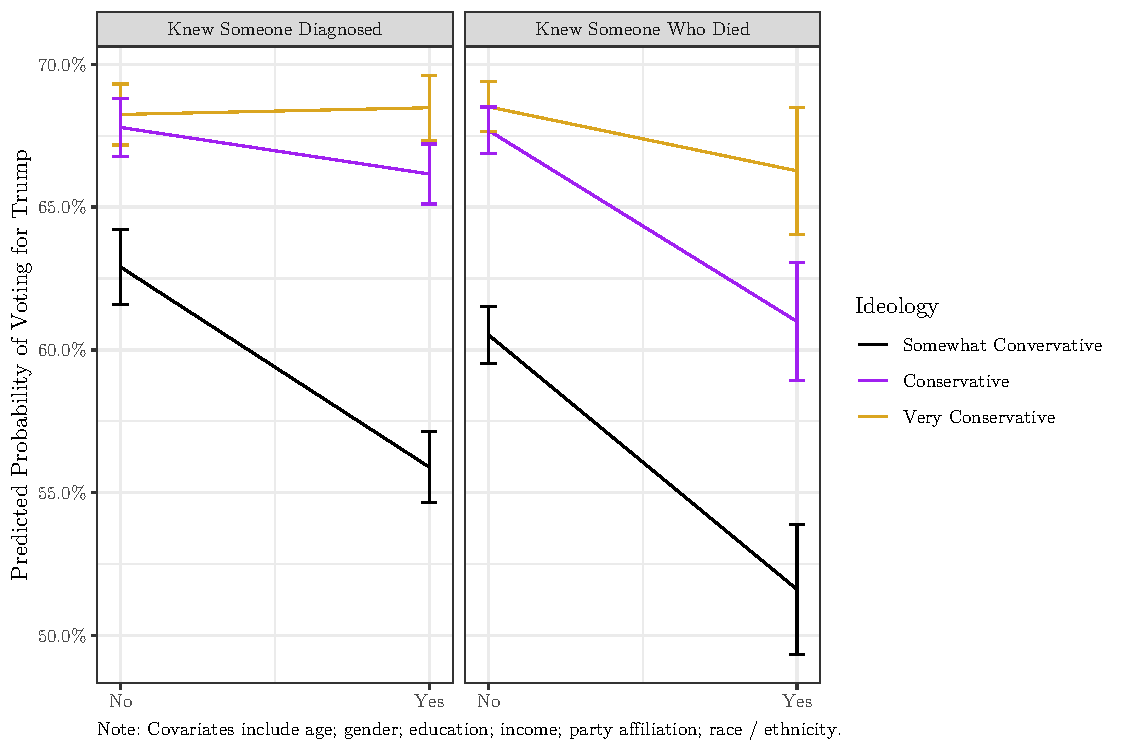
\includegraphics{theory_paper_files/figure-latex/mef3-c-1} 

}

\caption{\label{fig:mef3}Predicted Trump Support Among Conservative Participants, 2020 Election}\label{fig:mef3-c}
\end{figure}

Taken together, Figures \ref{fig:mef2} and \ref{fig:mef3} make clear the relationships between ideological commitments, COVID contact, and voting behavior in the 2020 election. Both the ``weak'' and ``strong'' treatments---knowing someone diagnosed with or who died from COVID-19, respectively---are associated with higher participation rates for weak conservatives. And not only were they more likely to vote---they also supported Trump at substantially lower rates. The salient threat of COVID-19, then, overrode any impulse to withdraw. The exact opposite is true of the very conservative respondents: these individuals were led to \emph{withdraw} from the political process due to their exposure to COVID-19, but COVID-19 contact \emph{did not impact} support for Trump among those who did participate (\emph{p} = 0.72 for knowing someone diagnosed, \emph{p} = 0.12 for knowing someone who died). Unsurprisingly, middle-of-the-road conservatives fell somewhere in between: the weak treatment was associated with withdrawal and unassociated with Trump support, while the strong treatment was unassociated with turnout but did lead to lower Trump support.

\hypertarget{discussion}{%
\section*{Discussion}\label{discussion}}
\addcontentsline{toc}{section}{Discussion}

As COVID-19 tore through the United States in 2020, it presented Republicans in contact with the virus a stark choice: would they continue to support the charismatic leader whose actions may have harmed them or their loved ones? Would they vote for the other party's candidate, perhaps violating an important part of their social identity? Or would they withdraw from the political process entirely, preferring not voting over supporting either Donald Trump or the Democratic Party? As discussed above, Émile Durkheim's conception of anomie as developed in \emph{Suicide} offers some insight, but ultimately leaves its central question unanswered: when does a great social disturbance arouse collective sentiments, and when does it lead to withdrawal?

This study begins to address that tension. The results are strong and unambiguous: the stronger one feels about their political orientation, the stronger the withdrawal in response to a failure of that political orientation. Very conservative voters were not roused to political participation in an effort to redefine conservatism or support a different candidate; instead, they abstained. In fact, abstention explains the entirety of their political response: support for Trump among very conservative respondents who voted and had contact with COVID-19 was no different than that of other very conservative participants. Respondents who identified as just somewhat conservative, however, \emph{did} see their collective sentiments roused in response to COVID-19: somewhat conservative voters with COVID-19 contact were considerably more likely to vote than somewhat conservatives without such contact, and were also far less likely to vote for Donald Trump.

This short study raises important questions about how strong group attachments can lead to \emph{disengagement}, the opposite of what we normally expect.

\newpage

\hypertarget{references}{%
\section*{References}\label{references}}
\addcontentsline{toc}{section}{References}

\hypertarget{refs}{}
\begin{CSLReferences}{1}{0}
\leavevmode\hypertarget{ref-Abrajano2017}{}%
Abrajano, Marisa A., and Zoltan Hajnal. 2017. \emph{White Backlash: Immigration, Race, and {American} Politics}. {Princeton Oxford}: {Princeton University Press}.

\leavevmode\hypertarget{ref-Bakker2016}{}%
Bakker, Bert N., Robert Klemmensen, Asbjørn Sonne Nørgaard, and Gijs Schumacher. 2016. {``Stay {Loyal} or {Exit} the {Party}? {How Openness} to {Experience} and {Extroversion Explain Vote Switching}.''} \emph{Political Psychology} 37 (3): 419--29. \url{https://doi.org/10.1111/pops.12257}.

\leavevmode\hypertarget{ref-Blais2001}{}%
Blais, André, Elisabeth Gidengil, Richard Nadeau, and Neil Nevitte. 2001. {``Measuring {Party Identification}: {Britain}, {Canada}, and the {United States}.''} \emph{Political Behavior} 23 (1): 5--22. \url{https://doi.org/10.1023/A:1017665513905}.

\leavevmode\hypertarget{ref-Bogel-Burroughs2020}{}%
Bogel-Burroughs, Nicholas, and Jeremy W. Peters. 2020. {``{`{You Have} to {Disobey}'}: {Protesters Gather} to {Defy Stay}-at-{Home Orders}.''} \emph{The New York Times: U.S.}, April 16, 2020. \url{https://www.nytimes.com/2020/04/16/us/coronavirus-rules-protests.html}.

\leavevmode\hypertarget{ref-Calia2020}{}%
Calia, Mike. 2020. {``Full Interview: {President Trump} Discusses Trade, Impeachment, {Boeing} and {Elon Musk} with {CNBC} in {Davos}.''} \emph{CNBC: Davos WEF}, January 22, 2020. \url{https://www.cnbc.com/2020/01/22/davos-2020-cnbcs-full-interview-with-president-trump.html}.

\leavevmode\hypertarget{ref-Dassonneville2015}{}%
Dassonneville, Ruth, André Blais, and Yves Dejaeghere. 2015. {``Staying {With} the {Party}, {Switching} or {Exiting}? {A Comparative Analysis} of {Determinants} of {Party Switching} and {Abstaining}.''} \emph{Journal of Elections, Public Opinion and Parties} 25 (3): 387--405. \url{https://doi.org/10.1080/17457289.2015.1016528}.

\leavevmode\hypertarget{ref-Douglas2020}{}%
Douglas, Jason. 2020. {``As {Coronavirus Surges} in {U}.{S}., {Some Countries Have Just About Halted It}.''} \emph{Wall Street Journal: World}, July 6, 2020. \url{https://www.wsj.com/articles/as-coronavirus-surges-in-u-s-some-countries-have-just-about-halted-it-11594037814}.

\leavevmode\hypertarget{ref-Fitzpatrick2020}{}%
Fitzpatrick, Alex. 2020. {``Why the {U}.{S}. {Is Losing} the {War On COVID}-19.''} \emph{Time}, August 13, 2020. \url{https://time.com/5879086/us-covid-19/}.

\leavevmode\hypertarget{ref-Golden2020}{}%
Golden, Hallie. 2020. {``Coronavirus: {Washington} State at Center of {US} Outbreak as 18 Cases Confirmed.''} \emph{The Guardian: World News}, March 3, 2020. \url{https://www.theguardian.com/world/2020/mar/02/washington-state-coronavirus-outbreak-nursing-home}.

\leavevmode\hypertarget{ref-Gonzales2019}{}%
Gonzales, Richard. 2019. {``{NOAA Contradicts Weather Service}, {Backs Trump On Hurricane Threat In Alabama}.''} \emph{NPR.org}, September 6, 2019. \url{https://www.npr.org/2019/09/06/758532041/noaa-contradicts-weather-service-backs-trump-on-hurricane-threat-in-alabama}.

\leavevmode\hypertarget{ref-Green2002}{}%
Green, Donald P, Bradley Palmquist, and Eric Schickler. 2002. \emph{Partisan Hearts and Minds: Political Parties and the Social Identities of Voters}. {New Haven, Conn.; London}: {Yale University Press}.

\leavevmode\hypertarget{ref-Hirschman1970a}{}%
Hirschman, Albert O. 1970. \emph{Exit, Voice, and Loyalty: Responses to Decline in Firms, Organizations, and States}. {Cambridge, Mass}: {Harvard University Press}.

\leavevmode\hypertarget{ref-Huddy2015}{}%
Huddy, Leonie, Lilliana Mason, and Lene Aarøe. 2015. {``Expressive {Partisanship}: {Campaign Involvement}, {Political Emotion}, and {Partisan Identity}.''} \emph{The American Political Science Review} 109 (1): 1--17. \url{http://www.jstor.org/stable/43655021}.

\leavevmode\hypertarget{ref-Iyengar2019}{}%
Iyengar, Shanto, Yphtach Lelkes, Matthew Levendusky, Neil Malhotra, and Sean J. Westwood. 2019. {``The {Origins} and {Consequences} of {Affective Polarization} in the {United States}.''} \emph{Annual Review of Political Science} 22 (1): 129--46. \url{https://doi.org/10.1146/annurev-polisci-051117-073034}.

\leavevmode\hypertarget{ref-Kolata2020}{}%
Kolata, Gina, and Roni Caryn Rabin. 2020. {``{`{Don}'t {Be Afraid} of {Covid},'} {Trump Says}, {Undermining Public Health Messages}.''} \emph{The New York Times: Health}, October 5, 2020. \url{https://www.nytimes.com/2020/10/05/health/trump-covid-public-health.html}.

\leavevmode\hypertarget{ref-Lu2020}{}%
Lu, Denise. 2020. {``The {True Coronavirus Toll} in the {U}.{S}. {Has Already Surpassed} 200,000.''} \emph{The New York Times: U.S.}, August 13, 2020. \url{https://www.nytimes.com/interactive/2020/08/12/us/covid-deaths-us.html}.

\leavevmode\hypertarget{ref-Mason2015}{}%
Mason, Lilliana. 2015. {``{`{I Disrespectfully Agree}'}: {The Differential Effects} of {Partisan Sorting} on {Social} and {Issue Polarization}.''} \emph{American Journal of Political Science} 59 (1): 128--45. \url{https://doi.org/10.1111/ajps.12089}.

\leavevmode\hypertarget{ref-Mason2018}{}%
---------. 2018. \emph{Uncivil Agreement: How Politics Became Our Identity}. {Chicago, Illinois ; London}: {The University of Chicago Press}.

\leavevmode\hypertarget{ref-McNerthney2020}{}%
McNerthney, Casey. 2020. {``Coronavirus in {Washington} State: {A} Timeline of the Outbreak Through {March} 2020.''} \emph{KIRO}, April 3, 2020. \url{https://www.kiro7.com/news/local/coronavirus-washington-state-timeline-outbreak/IM65JK66N5BYTIAPZ3FUZSKMUE/}.

\leavevmode\hypertarget{ref-Moon2020}{}%
Moon, Sarah. 2020. {``A Seemingly Healthy Woman's Sudden Death Is Now the First Known {US} Coronavirus-Related Fatality.''} \emph{CNN}, April 24, 2020. \url{https://www.cnn.com/2020/04/23/us/california-woman-first-coronavirus-death/index.html}.

\leavevmode\hypertarget{ref-nyt2020}{}%
\emph{New York Times: U.S.} 2020. {``Covid in the {U}.{S}.: {Latest Map} and {Case Count},''} November 3, 2020. \url{https://www.nytimes.com/interactive/2020/us/coronavirus-us-cases.html}.

\leavevmode\hypertarget{ref-Pope1975}{}%
Pope, Whitney. 1975. {``Concepts and {Explanatory Structure} in {Durkheim}'s {Theory} of {Suicide}.''} \emph{The British Journal of Sociology} 26 (4): 417--34. \url{https://doi.org/10.2307/589820}.

\leavevmode\hypertarget{ref-whitehouse2020}{}%
{``Remarks by {President Trump} at a {USMCA Celebration} with {American Workers} \textbar{} {Warren}, {MI}.''} 2020. {The White House}. January 30, 2020. \url{https://www.whitehouse.gov/briefings-statements/remarks-president-trump-usmca-celebration-american-workers-warren-mi/}.

\leavevmode\hypertarget{ref-Shear2016}{}%
Shear, Michael D., and Gardiner Harris. 2016. {``Trump {Wants} to {`{Drain} the {Swamp},'} but {Change Will Be Complex} and {Costly}.''} \emph{The New York Times: U.S.}, November 11, 2016. \url{https://www.nytimes.com/2016/11/11/us/politics/trump-government.html}.

\leavevmode\hypertarget{ref-Shear2020}{}%
Shear, Michael D., Noah Weiland, Eric Lipton, Maggie Haberman, and David E. Sanger. 2020. {``Inside {Trump}'s {Failure}: {The Rush} to {Abandon Leadership Role} on the {Virus}.''} \emph{The New York Times: U.S.}, July 18, 2020. \url{https://www.nytimes.com/2020/07/18/us/politics/trump-coronavirus-response-failure-leadership.html}.

\leavevmode\hypertarget{ref-Wan2020}{}%
Wan, William. 2020. {``{WHO} Declares a Pandemic of Coronavirus Disease Covid-19.''} \emph{Washington Post}, March 11, 2020. \url{https://www.washingtonpost.com/health/2020/03/11/who-declares-pandemic-coronavirus-disease-covid-19/}.

\end{CSLReferences}

\end{document}
